%You can leave alone everything before Line 79.
\documentclass{article}
\usepackage{url,amsfonts, amsmath, amssymb, amsthm,color, enumerate}
% Page layout
\setlength{\textheight}{8.75in}
\setlength{\columnsep}{2.0pc}
\setlength{\textwidth}{6.5in}
\setlength{\topmargin}{0in}
\setlength{\headheight}{0.0in}
\setlength{\headsep}{0.0in}
\setlength{\oddsidemargin}{0in}
\setlength{\evensidemargin}{0in}
\setlength{\parindent}{1pc}
\newcommand{\shortbar}{\begin{center}\rule{5ex}{0.1pt}\end{center}}
%\renewcommand{\baselinestretch}{1.1}
% Macros for course info
\newcommand{\courseNumber}{ME 552}
\newcommand{\courseTitle}{Mechatronics}
\newcommand{\semester}{Fall 2012}
\newcommand{\xxx}[1]{\textcolor{red}{#1}}
% Theorem-like structures are numbered within SECTION units
\theoremstyle{plain}
\newtheorem{theorem}{Theorem}[section]
\newtheorem{lemma}[theorem]{Lemma}
\newtheorem{corollary}[theorem]{Corollary}
\newtheorem{proposition}[theorem]{Proposition}
\newtheorem{statement}[theorem]{Statement}
\newtheorem{conjecture}[theorem]{Conjecture}
\newtheorem{fact}{Fact}
%definition style
\theoremstyle{definition}
\newtheorem{definition}[theorem]{Definition}
\newtheorem{example}{Example}
\newtheorem{problem}[theorem]{Problem}
\newtheorem{exercise}{Exercise}
\newtheorem{algorithm}{Algorithm}
%remark style
\theoremstyle{remark}
\newtheorem{remark}[theorem]{Remark}
\newtheorem{reduction}[theorem]{Reduction}
%\newtheorem{question}[theorem]{Question}
\newtheorem{question}{Question}
%\newtheorem{claim}[theorem]{Claim}
%
% Proof-making commands and environments
\newcommand{\beginproof}{\medskip\noindent{\bf Proof.~}}
\newcommand{\beginproofof}[1]{\medskip\noindent{\bf Proof of #1.~}}
\newcommand{\finishproof}{\hspace{0.2ex}\rule{1ex}{1ex}}
\def\therefore{\boldsymbol{\text{ }
\leavevmode
\lower0.4ex\hbox{$\cdot$}
\kern-.5em\raise0.7ex\hbox{$\cdot$}
\kern-0.55em\lower0.4ex\hbox{$\cdot$}
\thinspace\text{ }}}

\newenvironment{solution}[1]{\medskip\noindent{\bf Problem #1.~}}{\shortbar}

%====header======
\newcommand{\solutions}[4]{
%\renewcommand{\thetheorem}{{#2}.\arabic{theorem}}
\vspace{-2ex}
\begin{center}
{\small  \courseNumber, \courseTitle
\hfill {\Large \bf {#1} }\\
\semester, University of Michigan, Ann Arbor \hfill
{\em Date: #3}}\\
\vspace{-1ex}
\hrulefill\\
\vspace{4ex}
{\LARGE Lab Assignment #2}\\
\vspace{2ex}
\end{center}
\begin{trivlist}
\item \textsc{Team members:\\} {#4}
\end{trivlist}
\noindent
\shortbar
\vspace{3ex}
}
% math macros
\newcommand{\defeq}{\stackrel{\textrm{def}}{=}}
\newcommand{\Prob}{\textrm{Prob}}
%==
\usepackage{graphicx}
\usepackage{xfrac}
\usepackage{amsmath}
\begin{document}
%%%%%%%%%%%%%%%%%%%%%%%%%%%%%%%%%%%%%%%%%%%%%%%%%
%\solutions{Your name}{Problem Set Number}{Date of preparation}{Collaborators}{Prover}{Verifiers}
\solutions{}{2: MagLev}{\today}{Shiva Ghose, @gshiva\\ John Peterson, @jrpeters\\ Peter Turpel, @pturpel\\ Chan-Rong Lin, @pmelin}
%%%%%%%%%%%%%%%%%%%%%%%%%%%%%%%%%%%%%%%%%%%%%%%%%
%\renewcommand{\theproblem}{\arabic{problem}} 
%%%%%%%%%%%%%%%%%%%%%%%%%%%%%%%%%%%%%%%%%%%%%%%%%
%
% Begin the solution for each problem by
% \begin{solution}{Problem Number} and ends it with \end{solution}
%
% the solution for Problem 
\section*{Teamwork Participation Pledge :: Team 1}

I attest that I have made a fair and equitable contribution to this lab and submitted 
assignment. \\

My signature also indicates that I have followed the University of Michigan Honor Code, 
while working on this lab and assignment.\\

I accept my responsibility to look after all of the equipment assigned to me and my team, 
and that I have read and understood the X50 Lab Rules.\\

\begin{table}[h]
\begin{center}
    \begin{tabular}{|c|c|c|}
        \hline
        \textbf{Name} & \textbf{Email}     & \textbf{ \ \ \ \ \  \ \  \ \ \ \ \  \ \ Signature  \ \ \ \ \  \ \ \ \ \ \ \  \ \ } \\ \hline
        	~& ~& ~\\
	~& ~& ~\\
	Shiva Ghose   & gshiva@umich.edu   & ~                  \\
	~& ~& ~\\
	~& ~& ~\\ \hline 
	~& ~& ~\\
	~& ~& ~\\
        John Peterson & jrpeters@umich.edu & ~                  \\ 
	~& ~& ~\\
	~& ~& ~\\ \hline 
	~& ~& ~\\
	~& ~& ~\\
        Peter Turpel   & pturpel@umich.edu & ~                  \\
	~& ~& ~\\
	~& ~& ~\\ \hline 
	~& ~& ~\\
	~& ~& ~\\
        Chan-Rong Lin   & pmelin@umich.edu & ~                  \\
	~& ~& ~\\
	~& ~& ~\\ \hline 
        \hline
    \end{tabular}
\end{center}
\end{table}

\newpage
\begin{center}
\section*{Part B}
\end{center}
\section*{Question 1}

\subsection*{a.}

\subsubsection*{Break Beam Sensor}

\textbf{Assumptions} 
\begin{itemize}
\item Neglect the effects of diffraction.
\item Light rays are parallel. 
\item Neglect reflection of IR light by the polished ball stand.
\end{itemize}
As a consequence of these assumptions the IR beam from the LED to the photo-transistor can be modeled as a cylinder with a radius approximately equal to the radius of the phototransistor.  The shadow cast by the sphere is then simply a circle with radius equal to the radius of the sphere blocking part of the cross section of the beam.  These assumptions also mean that the distance between the sphere and the IR LED does not matter.  The only values that matter are the radius of the IR beam, the radius of the sphere, and the perpendicular distance between the axis of the beam and the center of the sphere.  The amount of light received by the photo-transistor can then simply be modeled as the intersection of two circles in 2-dimensions as shown in figure \ref{Q1_a1}. \\

\[
  Radiance \hspace{0.1cm} Fraction = \left\{
  \begin{array}{l l}
    \frac{A_{beam} - A_{sphere}}{A_{beam}} & \quad \text{if } r_{sphere} + |d| < r_{beam} \\
    0 & \quad \text{if } r_{beam} + |d| < r_{sphere} \\
    1 & \quad \text{if } |d| < r_{beam} + r_{sphere} \\
    \frac{A_{beam} - A_{Overlap}}{A_{beam}} & \quad \text{if } |d| < r_{sphere} + r_{beam} \\
  \end{array} \right.
\]

\textbf{Where:}
$$ A_{beam} = \pi r_{beam}^2$$
$$A_{sphere} = \pi r_{sphere}^2 $$ 
$$ y = \frac{d^2+r_{beam}^2-r_{sphere}^2}{2d}$$
$$ d_{beam}=y$$
$$ d_{sphere}=d-y=\frac{d^2-r_{beam}^2+r_{sphere}^2}{2d} $$
$$ A_{Obeam} = r_{beam}^2 \cos^{-1} (\frac{d_{beam}}{r_{beam}})-d_{beam} \sqrt{r_{beam}^2-d_{beam}^2}$$ 
$$ A_{Osphere} = r_{sphere}^2 \cos^{-1} (\frac{d_{sphere}}{r_{sphere}})-d_{sphere} \sqrt{r_{sphere}^2-d_{sphere}^2}$$
$$ A_{Overlap} = A_{Obeam} + A_{Osphere} $$

\begin{figure}
\begin{center}
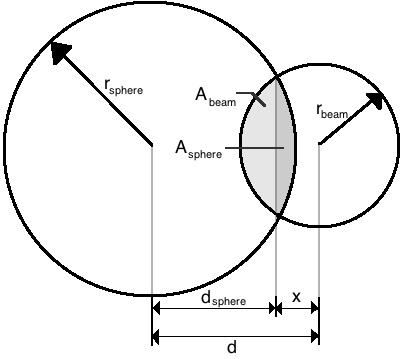
\includegraphics[width = 9cm]{beam_sphere_diagram.png}
\caption{\emph{Planar approximation of IR beam occluded by steel sphere}}
\label{Q1_a1}
\end{center}
\end{figure}

\subsubsection*{Driver Circuit}
\textbf{Assumptions}
\begin{itemize}
\item Op-Amp Golden Rules: voltage at inverting and non-inverting terminals is equal and op-amp input impedance is infinite
\end{itemize}

The electromagnet driver is a simple op-amp circuit, shown in figure \ref{Q1_a2}, which is designed to pass a specific current through the electromagnet for a a given input voltage.  The voltage at the non-inverting input can be simply determined by applying the voltage divider rule.  The voltage at the inverting input is now known allowing us to apply Ohm's Law to determine the current through $R_{3}$ and therefore through the electromagnet.  Notice that the resistance of the electromagnet does not affect the current provided by the driver circuit.

$$ V^{+}=\frac{R_2}{R_1+R_2}V_{in} \hspace{1cm} I_{EM}=\frac{V^{+}}{R_3}=\frac{1}{R_3}\left(\frac{R_2}{R_1+R_2}\right)V_{in} = DV_{in}$$

\begin{figure}
\begin{center}
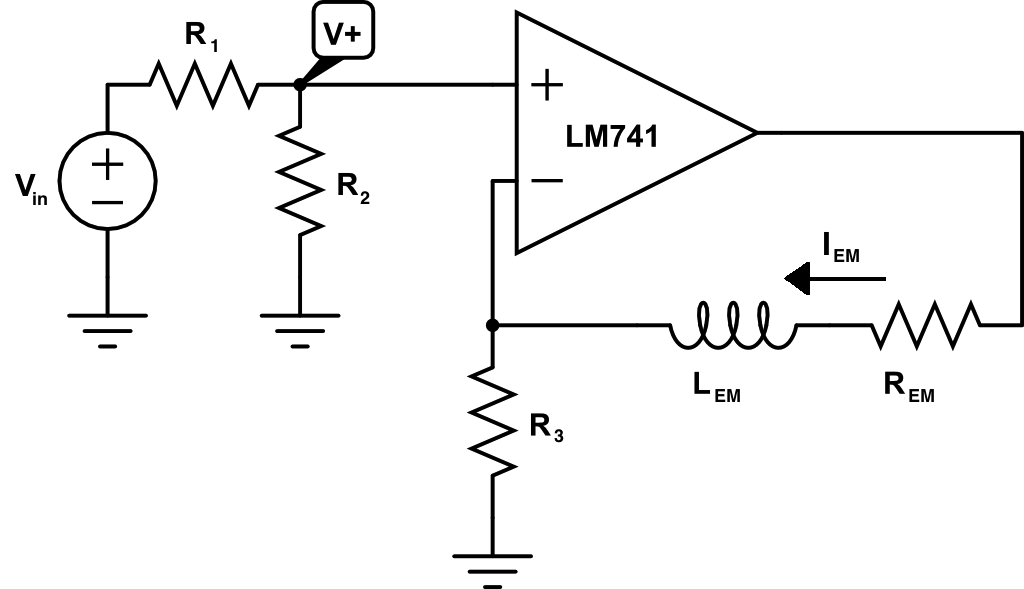
\includegraphics[width = 9cm]{em_driver_circuit.png}
\caption{\emph{Electromagnet Driver Circuit}}
\label{Q1_a2}
\end{center}
\end{figure}

\subsubsection*{Electromagnet}
\textbf{Assumptions}

\begin{figure}[htb]
\begin{minipage}[b]{0.45\linewidth}
\centering
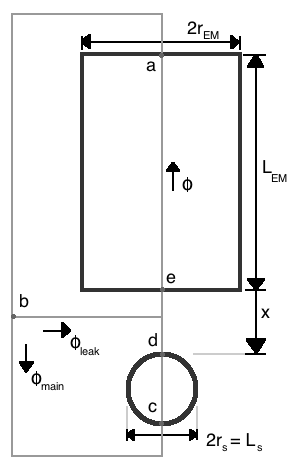
\includegraphics[width = 7cm]{flux_diagram.png}
\caption{\emph{Approximate Flux paths taken through our system}}
\label{Q1_a3L}
\end{minipage}
\hspace{0.5cm}
\begin{minipage}[b]{0.45\linewidth}
\centering
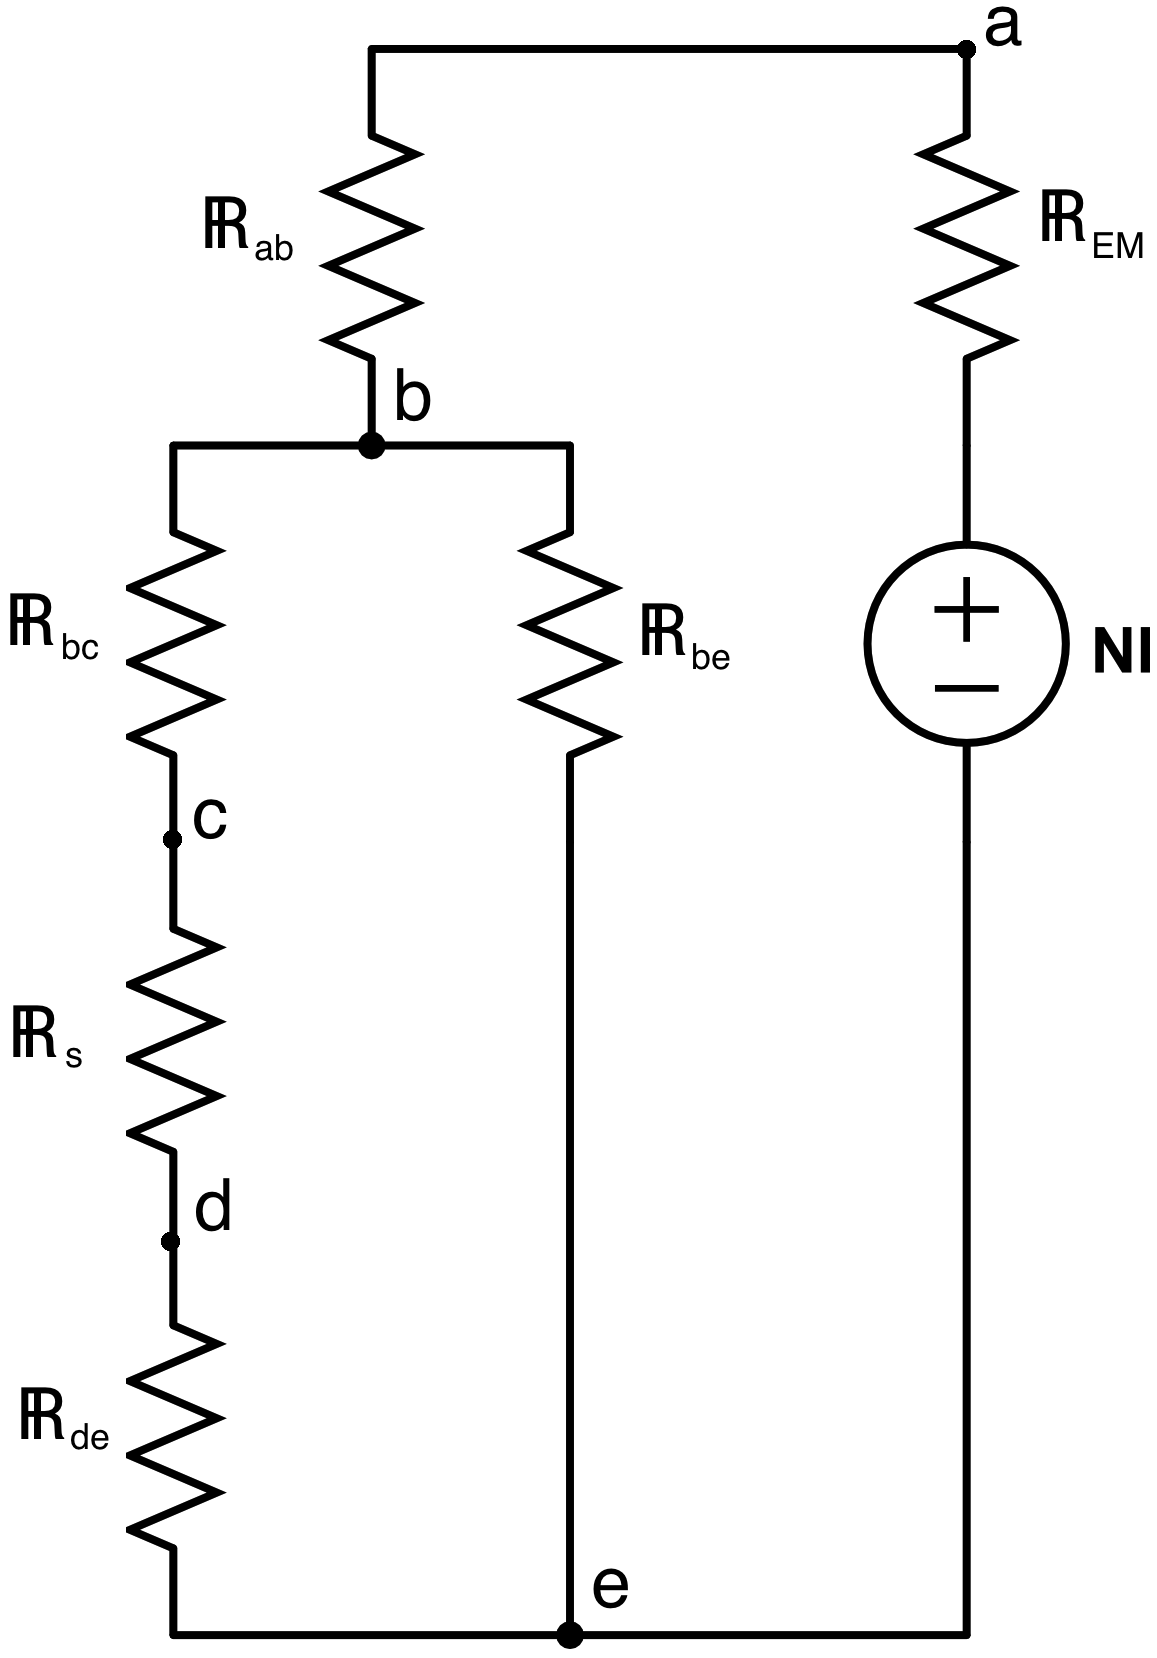
\includegraphics[width = 8cm]{magnetic_circuit.png}
\caption{\emph{Equivalent Magnetic Circuit}}
\label{Q1_a3R}
\end{minipage}
\end{figure}

\begin{itemize}
\item $ \mu_{Al} \approx \mu_{Cu} \approx \mu_{air} $ , where $\mu_x$ is the absolute permeability of material $x$
\item $ \mu_{steel} \gg \mu_{air} $
\item We can model the steel sphere as a cylinder with its axis collinear with the electromagnet  \\ 
$$A_{cd} \approx A_{s} = \pi * r_{sphere}^2 $$ 
\item We can neglect the effects of fringing on the cross-sectional area of paths through the air and assume particular dimensions that are consistent with the solid objects in the system \\
$$ A_{EM} = \pi*r_{EM}^2 \approx A_{ab} \hspace{1cm} A_{s} \approx A_{bc} \approx A_{de} \hspace{1cm} A_{EM} \approx A_{be} + A_{bc} $$ 
\item Path length from b to c (see figure \ref{Q1_a2}) does not vary with x: 
$ \frac{\partial}{\partial x} (L_{bc}) = 0$
\item The sphere remains in line with the axis of the electro magnet and in front of the magnet $( x > 0 )$
\end{itemize}

Drawing out approximate flux paths yields the diagram in figure \ref{Q1_a3L}, which can be converted to an equivalent magnetic circuit, shown in figure \ref{Q1_a3R}, by applying Ampere's Law and Maxwell's $2^{nd}$ law resulting in the following three equations. 

$$ NI = \phi \left (\mathbb{R}_{EM} + \mathbb{R}_{ab}\right) + \phi_{main} \left( \mathbb{R}_{bc}+\mathbb{R}_{s}+\mathbb{R}_{dc} \right) $$
$$ NI = \phi \left( \mathbb{R}_{EM} + \mathbb{R}_{ab} \right) + \phi_{leak} \left( \mathbb{R}_{be} \right) $$
$$ \phi = \phi_{main} + \phi_{leak} $$


$$ \mathbb{R}_{EM} = \frac{L_{EM}}{A_{EM}\mu_{air}}  \hspace{1cm} \mathbb{R}_{ab} = \frac{L_{ab}}{A_{EM}\mu_{air}} \hspace{1cm} \mathbb{R}_{bc} = \frac{L_{bc}}{(A_{s})\mu_{air}} \hspace{1cm} \mathbb{R}_{de} = \frac{x}{A_{A_{s}}\mu_{air}} \hspace{1cm} $$ $$ \mathbb{R}_{be} = \frac{L_{be}}{(A_{EM} - A_{s})\mu_{air}}  \hspace{1cm}  \mathbb{R}_{s} = \frac{2*r_{sphere}}{A_{s}\mu_{steel}} \approx 0$$

Solving the $2^{nd}$ equation for $\phi_{leak}$ gives:

$$\phi_{leak} = C_{0}\left( NI-C_{1}\phi_{main} \right)$$ 
$$C_{0} = \frac{\mu_{air} A_{EM} (A_{EM} - A_{s})}{L_{be} A_{EM} + (L_{EM} + L_{ab})(A_{EM} - A_{s}))} \hspace{1cm} 
C_{1} = \frac{L_{EM} + L_{ab}}{\mu_{air} A_{EM}} $$

Substituting back into the $1^{st}$ equation lets us solve for $\phi_{main}$ yielding: 

$$ \phi_{main} = \frac{NI(1-C_{0}C_{1})}{C_{1} - C_{0} C_{1}^2 + \frac{L_{bc}}{\mu_{air} A_{s}} + \frac{x}{\mu_{air} A_{s}}} $$

With equations for our fluxes, we can now compute the self inductance and from that compute the force exerted on the steel sphere as a function of position and current.

$$ \lambda = N \phi = L(x) I $$
$$ W(i,x) = (\sfrac{1}{2}) L(x) I^2 = (\sfrac{1}{2}) N \phi(x) I =(\sfrac{1}{2}) N I (\phi_{main}(x) + \phi_{leak}(x))$$
$$ F(i,x) = \frac{d}{dx} (W(i,x) )= (\sfrac{1}{2}) N I ( \frac{d}{dx} (\phi_{main}) + \frac{d}{dx} (\phi_{leak})) $$

$$ \frac{d}{dx}(\phi_{main}) = - \frac{N I (1 - C_{0}C_{1} \mu_{air} A_{s}}{(\mu_{air} A_{s}(C_{1} - C_{0} C_{1}^2 + C_{2}) + x)^2} dx$$

$$ \frac{d}{dx}(\phi_{leak}) = -C_{0} C_{1} \frac{d}{dx}(\phi_{main})$$

Combining terms yields our final expression for the force.

$$ F_{EM}(x) = -\frac{1}{2} \left( 1 - C_{0}C_{1} \right)^2 \frac{\mu_{air} A_{s} N^2 }{(\mu_{air} A_{s}(C_{1} - C_{0} C_{1}^2 + C_{2}) + x)^2} I^2 $$

We can then condense these terms to arrive at a simple equation to model the force, shown below.  Where values for A and B can be obtained experimentally.

$$ F_{EM}(x) = -\frac{A I^2}{(B+x)^2} $$

\subsubsection*{Steel Sphere \& Magnet System}
\textbf{Assumptions}
\begin{itemize}
\item Air resistance is negligible.
\item The steel sphere does not collide with the magnet: $x > 0$
\end{itemize}

According to Newton's second law the sum of the forces on an object is proportional to the acceleration of the object.  After constructing a free body diagram of our system shown in figure \ref{Q1_a4} we can very easily derive a model of the motion of our system.

$$ \sum F_x = mg + F_{EM} = mg -\frac{A I^2}{(B+x)^2} = m  \ddot{x}$$

\begin{figure}
\begin{center}
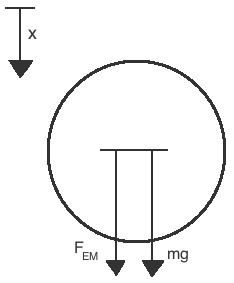
\includegraphics[width = 5cm]{freebodydiagram.png}
\caption{\emph{Free body diagram of steel sphere.  Note: The x axis points downwards and our force was computed according to this convention, which is why their is a negative sign in the expression of the force generated by the electromagnet.}}
\label{Q1_a4}
\end{center}
\end{figure}

\subsection*{b.}
\subsubsection*{Break Beam Sensor}
The position sensor is very nearly linear over the range of positions that we are concerned with but does saturate for small and large values for x.  To linearize the sensor we must perform a 1st order Taylor approximation which requires the derivative of the function about the nominal value.  The numerical derivative is easily obtained, but the symbolic computation of the derivative, shown below, is far more involved. 

$$ d = x + 4.12 \hspace{1cm} \partial x=\partial d $$
$$ y = \frac{d^2+r_{beam}^2-r_{sphere}^2}{2d}=\frac{d}{2} + \frac{r_{beam}^2}{2d} - \frac{r_{sphere}^2}{2d} \hspace{1cm} \frac{\partial}{\partial d} y = \left(\frac{1}{2}  -\frac{r_{beam}^2}{2d^2} + \frac{r_{sphere}^2}{2d^2}\right) \partial d $$
$$ d_{beam}=y \hspace{1cm} \frac{\partial}{\partial d} d_{beam} =  \frac{\partial}{\partial d} y = \left(\frac{1}{2}  -\frac{r_{beam}^2}{2d^2} + \frac{r_{sphere}^2}{2d^2}\right) \partial d $$
$$  d_{sphere}=d-y \hspace{1cm}   \frac{\partial}{\partial d} d_{sphere} = 1\partial d - \frac{\partial}{\partial d} y = \left(1 - \frac{1}{2}  +\frac{r_{beam}^2}{2d^2} - \frac{r_{sphere}^2}{2d^2}\right) \partial d = \left(\frac{1}{2}  +\frac{r_{beam}^2}{2d^2} - \frac{r_{sphere}^2}{2d^2}\right) \partial d$$
$$ A_{Obeam} = r_{beam}^2 \cos^{-1} (\frac{d_{beam}}{r_{beam}})-d_{beam} \sqrt{r_{beam}^2-d_{beam}^2}$$ 

$$ \frac{\partial}{\partial d} A_{Obeam} = \left( -\frac{r_{beam}}{\sqrt{1 - \left(\frac{d_{beam}}{r_{beam}}\right)^2}} - \left( r_{beam}^2 - d_{beam}^2\right)^{\sfrac{1}{2}} + d_{beam}^2 \left( r_{beam}^2 - d_{beam}^2\right)^{\sfrac{-1}{2}} \right) \frac{\partial d_{beam}}{\partial d}$$

$$ A_{Osphere} = r_{sphere}^2 \cos^{-1} (\frac{d_{sphere}}{r_{sphere}})-d_{sphere} \sqrt{r_{sphere}^2-d_{sphere}^2} $$

$$ \frac{\partial}{\partial d} A_{Osphere} = \left( -\frac{r_{sphere}}{\sqrt{1 - \left(\frac{d_{sphere}}{r_{sphere}}\right)^2}} - \left( r_{sphere}^2 - d_{sphere}^2\right)^{\sfrac{1}{2}} + d_{sphere}^2 \left( r_{sphere}^2 - d_{sphere}^2\right)^{\sfrac{-1}{2}} \right) \frac{\partial d_{sphere}}{\partial d}$$

$$ A_{Overlap} = A_{Obeam} + A_{Osphere} \hspace{1cm}  \frac{\partial}{\partial d} A_{Overlap} = \frac{\partial}{\partial d} A_{Obeam} + \frac{\partial}{\partial d} A_{Osphere} $$

The set point we are linearizing about is in the area where the function above is well behaved:

$$ Radiance \hspace{0.1cm} Fraction = \frac{A_{beam} - A_{Overlap}}{A_{beam}} = 1 - \frac{A_{Overlap}}{A_{beam}} \hspace{1cm} $$

$$ \frac{\partial}{\partial d} \left( Radiance \hspace{0.1cm} Fraction \right) = \frac{1}{A_{beam}} \left( \frac{\partial}{\partial d} A_{Overlap} \right) $$

Taylor expansion allows us to approximate the Radiance Fraction about a certain distance $d_0$ as:

$$ Radiance \hspace{0.1cm} Fraction = R(d) = R(d_{0}) + \left. \frac{\partial \, R(d)}{\partial d} \right|_{d_{0}} \left( d - d_{0} \right) + \left. \frac{1}{2!} \frac{\partial^2 \, R(d)}{\partial d^2} \right|_{d_{0}} \left(d-d_{0}\right)^2 + ... $$

Dropping the higher order terms leaves us with a linear expression for the Radiance Fraction about a certain distance.

$$ R(d) \approx R(d_{0}) + \left. \frac{\partial \, R(d)}{\partial d} \right|_{d_{0}} \left( d - d_{0} \right) $$

Substituting our expression for d in terms of x yields:

$$ R(x) \approx R(x_{0} + 4.12) + \left. \frac{\partial \, R(x)}{\partial x} \right|_{x_{0}+4.12} \left( x - x_{0} \right) $$

Substituting our previous expressions in to obtain a single symbolic linear expression for the Radiance Fraction in terms of $x$, $r_{beam}$ and $r_{sphere}$ is possible but not particularly practical.  The appendix includes MATLAB code for computing $R'(d_{0})$ by computing numerical values for terms before performing the substitution.

To obtain the final expected voltage as a function of x, it is necessary to multiply by the full scale range, in our case 10 volts.


%$$ R(d) \approx \left(1 - \frac{A_{Overlap}(d_{0})}{A_{beam}} \right) + \frac{1}{A_{beam}} \left( \frac{\partial}{\partial d} A_{Overlap}(d_{0}) \right) \left(d - d_{0} \right)$$
%
%$$ R(d) \approx \left(1 - \frac{1}{A_{beam}}\left(A_{Obeam}(d_{0}) + A_{Osphere}(d_{0}) \right) \right) + \frac{1}{A_{beam}} \left( \frac{\partial}{\partial d} A_{Obeam}(d_{0}) + \frac{\partial}{\partial d} A_{Osphere}(d_{0}) \right) \left(d - d_{0} \right)$$
%
%\begin{multline}
%R(d) \approx \left(1 - \frac{1}{A_{beam}}\left(r_{beam}^2 \cos^{-1} (\frac{d_{beam}}{r_{beam}})-d_{beam} \sqrt{r_{beam}^2-d_{beam}^2} \right. \right. \\ \left. \left.+ r_{sphere}^2 \cos^{-1} (\frac{d_{sphere}}{r_{sphere}})-d_{sphere} \sqrt{r_{sphere}^2-d_{sphere}^2} \right) \right) \\ + \frac{1}{A_{beam}} \left( \left( -\frac{r_{beam}^2}{\sqrt{1 - \left(\frac{d_{beam}}{r_{beam}}\right)^2}} - \left( r_{beam}^2 - d_{beam}^2\right)^{\sfrac{1}{2}} - d_{beam}^2 \left( r_{beam}^2 - d_{beam}^2\right)^{\sfrac{1}{2}} \right) \frac{\partial d_{beam}}{\partial d} \right. \\ \left. +  \left( -\frac{r_{sphere}^2}{\sqrt{1 - \left(\frac{d_{sphere}}{r_{sphere}}\right)^2}} - \left( r_{sphere}^2 - d_{sphere}^2\right)^{\sfrac{1}{2}} - d_{sphere}^2 \left( r_{sphere}^2 - d_{sphere}^2\right)^{\sfrac{1}{2}} \right) \frac{\partial d_{sphere}}{\partial d} \right) \left(d - d_{0} \right)
%\end{multline}
%
%\begin{multline}
%R(d) \approx \left(1 - \frac{1}{A_{beam}}\left(r_{beam}^2 \cos^{-1} (\frac{d_{beam}}{r_{beam}})-d_{beam} \sqrt{r_{beam}^2-d_{beam}^2} \right. \right. \\ \left. \left.+ r_{sphere}^2 \cos^{-1} (\frac{d_{sphere}}{r_{sphere}})-d_{sphere} \sqrt{r_{sphere}^2-d_{sphere}^2} \right) \right) \\ + \frac{1}{A_{beam}} \left( \left( -\frac{r_{beam}^2}{\sqrt{1 - \left(\frac{d_{beam}}{r_{beam}}\right)^2}} - \left( r_{beam}^2 - d_{beam}^2\right)^{\sfrac{1}{2}} - d_{beam}^2 \left( r_{beam}^2 - d_{beam}^2\right)^{\sfrac{1}{2}} \right) \frac{\partial d_{beam}}{\partial d} \right. \\ \left. +  \left( -\frac{r_{sphere}^2}{\sqrt{1 - \left(\frac{d_{sphere}}{r_{sphere}}\right)^2}} - \left( r_{sphere}^2 - d_{sphere}^2\right)^{\sfrac{1}{2}} - d_{sphere}^2 \left( r_{sphere}^2 - d_{sphere}^2\right)^{\sfrac{1}{2}} \right) \frac{\partial d_{sphere}}{\partial d} \right) \left(d - d_{0} \right)
%\end{multline}

\subsubsection*{Electromagnet \& Steel Sphere}
We can model the dynamic forces of attraction between the ball and the magnet as follows:

$$\Sigma F_x = mg - \frac{A i^2}{(B + x)^2} = m\ddot{x}$$

\textbf{Where:}
$$ mg - \text{is the weight of the ball pulling downwards in the positive x direction}$$
$$- \frac{A i^2}{(B + x)^2} - \text{is the non-linear attractive force exerted by the electromagnet}$$
$$ m\ddot{x} - \text{is the net force experienced by the ball}$$

In order to simplify the system we would like to linearize the force of attraction exerted by the magnet around an equilibrium value. This can be achieved using the Taylor series expansion which allows us to represent the function as a sum of derivatives about the point of interest. The Taylor series of a function $f(a)$ is given by:
$$\sum_{n=0}^{\infty} \frac {f^{(n)}(a)}{n!} \, (x-a)^{n}$$
Which can be expanded to give:
$$f(a)+\frac {f'(a)}{1!} (x-a)+ \frac{f''(a)}{2!} (x-a)^2+\frac{f^{(3)}(a)}{3!}(x-a)^3+ \cdots.$$
Estimating the system up to the first derivative gives us sufficient approximation and results in a linear model.  We see that:
$$\frac{A i^2}{(B + x)^2} \approx \frac{A \bar{i}^2}{(B + \bar{x})^2} - 2\frac{A \bar{i}^2}{(B + \bar{x})^3}\hat{x} + 2\frac{A \bar{i}}{(B + \bar{x})^2}\hat{i}$$
\textbf{Where:}
$$\bar{i}- \text{is the current flowing through the electromagnet at equilibrium}$$
$$\hat{i}- \text{is the instantaneous current flowing through the electromagnet at the present time}$$
$$\bar{x}- \text{is the displacement of the ball from the electromagnet at equilibrium}$$
$$\hat{x}- \text{is the current displacement of the ball from it's equilibrium position.}$$

The expression for the forces acting on the ball can be rewritten as:
$$mg - \Big( \frac{A \bar{i}^2}{(B + \bar{x})^2} - 2\frac{A \bar{i}^2}{(B + \bar{x})^3}\hat{x} + 2\frac{A \bar{i}}{(B + \bar{x})^2}\hat{i} \Big) = m\ddot{\hat{x}}$$

At equilibrium the ball experiences zero net force along the vertical axis as the weight of the ball is negated by the equilibrium force of the magnet by definition.
$$mg = \frac{A \bar{i}^2}{(B + \bar{x})^2} $$
About the equilibrium point, the force acting on the ball can be rewritten as:
$$m\ddot{\hat{x}} = + 2\frac{A \bar{i}^2}{(B + \bar{x})^3}\hat{x} - 2\frac{A \bar{i}}{(B + \bar{x})^2}\hat{i}$$
Taking the Laplace transform of the expression, we get:
$$s^2 m \hat{X}(s) = + 2\frac{A \bar{i}^2}{(B + \bar{x})^3}\hat{X}(s) - 2\frac{A \bar{i}}{(B + \bar{x})^2}\hat{I}(s)$$
Grouping similar terms, we get:
$$\hat{X}(s) \Big( s^2 m - \frac{2A\bar{i}}{(B + \bar{x})^3} \Big) = \hat{I}(s) \Big( - \frac{2A\bar{i}}{(B + \bar{x})^2}\Big)$$
We can further rearrange the terms to get a ratio of the output to input as follows:
$$\frac{\hat{X}(s)}{\hat{I}(s)} = \frac{-2 A \bar{i} (B + \bar{x})}{s^2 (m (B + \bar{x})^3) - 2 A\bar{i}^2}$$
This is the linearized transfer function of the electromagnet-ball system. \\

\subsubsection*{Overall Linear Model}
Combining these linearized components allows us to compose an overall linear open loop transfer function from the plant and actuator, the driver circuit, and the sensor:
$$ \left(\frac{-2 A \bar{i} (B + \bar{x})}{m(B+\bar{x})^3 s^2 - 2 A \bar{i}^2}\right) \left(\frac{R_2}{R3(R1+R2)}\right)*\frac{\partial R}{\partial x} $$

Note that the specific values are explored later in the parameter identification section.

\subsection*{c.}
The sensor has a non-linear relationship between sphere position and output voltage.  The primary non-linearity in this system are the two saturations, at zero volts and the full scale value of 10 volts, which occur when the sphere is completely occluding the beam or completely out of the beam respectively.  The central region is non-linear, but is well approximated by a linear function.  Linear Controls theory may only be strictly applied to linear systems, because the Laplace Transform assumes linear time invariant systems.  Because of this assumption we must linearize our sensor about some nominal position.  The whole notion of a transfer function does not apply to a non-linear system so attempting to apply Linear Controls without the linearizion would be an oversight at best, if the system is pretty close to linear, or a complete disaster if it is not.  This non-linearity will cause the actual closed loop response to deviate from the results we would expect given the systems transfer function as we deviate from the nominal position.

\subsection*{d. Parameter Identification}

\subsubsection*{Break Beam Sensor}
To determine the model parameters of the break beam sensor model, the beam radius and the effective sphere radius, we acquired data measuring the relationship between the displacement between the optical axis of the phototransistor and the steel sphere and sensor voltage.  We sat the sphere on top of the stand and changed the height of the sphere stand and the magnet stand by known amounts, recording the voltage from the phototransistor at each displacement value.  Theoretically we would expect the beam radius to be very close to the radius of the phototransistor while we would expect the blocking radius to be very close to the radius of the sphere.  Non-linear optimization of the model revealed that that the actual values, shown in table \ref{Q1_dt1} were reasonably close to our expected values.  The curve resulting from this fit plotted alongside our data is shown in figure \ref{Q1_d1}.

\begin{table}
\begin{center}
    \begin{tabular}{|c|c|c|}
        \hline
        ~      & Expected Radii (mm) & Fit Radii (mm) \\ \hline
        Rbeam  & 2.3650              & 1.398935       \\ 
        Rblock & 6.350               & 6.070821       \\
        \hline
    \end{tabular}
\caption{\emph{Expected and Fit values for beam radius and blocking radius}}
\label{Q1_dt1}
\end{center}
\end{table}

\begin{figure}
\begin{center}
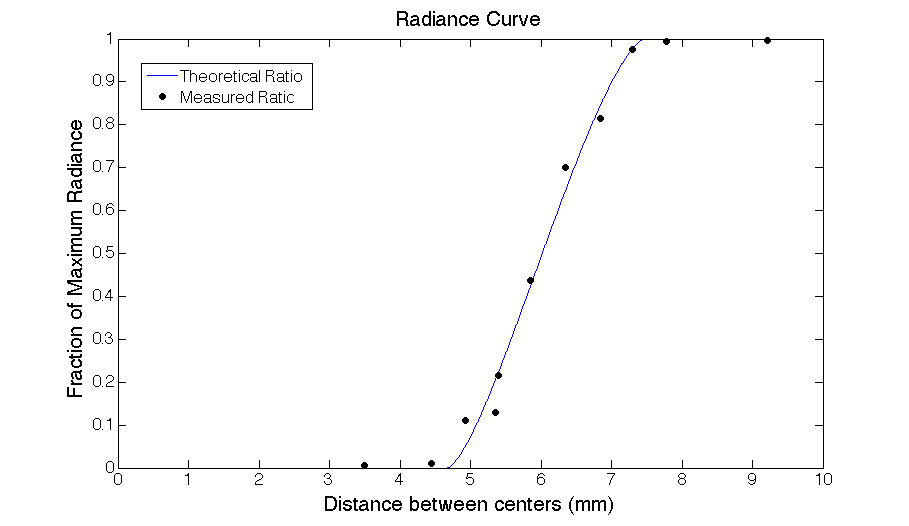
\includegraphics[width = 15cm]{SensorRadianceCurve.png}
\caption{\emph{Normalized Sensor Voltage Output vs distance from the optical axis}}
\label{Q1_d1}
\end{center}
\end{figure}

There is a fixed offset between the displacement, measured from the optical axis of the phototransistor to the center of the sphere, used in figure \ref{Q1_d1}, from the x, measured from the bottom of the magnet to the top of the sphere, used in our controller.  This relationship can be obtained by examining the physical dimensions of the system, noted in table \ref{Q1_dt2} yielding the following expression for x in terms of d.

$$ x = \Delta + h_{magnet} - h_{s stand} - r_{s} \hspace{1cm} \Delta = d + h_{s stand} - h_{sensor} $$

Evaluating this equation and solving for $x$ yields the following relationship:

$$ x = d - 4.12 \text{ mm} $$

\begin{table}
\begin{center}
    \begin{tabular}{|c|c|}
        \hline
        ~                                    & Dimension (mm) \\ \hline
        Magnet Height $(h_{magnet}) $          & 130.73         \\ 
        Sphere on Stand Height $(h_{s stand})$ & 121.5          \\ 
        Sensor Height $(h_{sensor})$           & 128.5          \\ 
        Sphere Radius $(r_{s})$                & 6.35           \\
        \hline
    \end{tabular}
\caption{\emph{Physical Dimensions of the System}}
\label{Q1_dt2}
\end{center}
\end{table}

\subsubsection*{Driver Circuit}

Theoretically the conversion from voltage to current for this system should be very straight forwards.  We used a multi-meter to measure the resistances, noted in table \ref{Q1_dt3}, and then plugged these values into our model yielding the following relationship between current and input voltage.

$$ I_{EM Expected}=\frac{1}{R_3}\left(\frac{R_2}{R_1+R_2}\right)V_{in} = \frac{1}{0.5 \,\Omega}\left(\frac{999 \,\Omega}{42.3 \,k\Omega + 999 \,\Omega}\right)V_{in} = 0.04233 \, V_{in}$$

However an examination of the actual current and voltage relationship revealed that the above relationship did not hold.  These current measurements were obtained obtained by using the current measuring functionality of the multi-meter.  Our observations revealed a steady state current even when the input voltage was 0, so we fit a more general linear model to the data excluding the input voltages above the current saturation.  It is also worth noting that we expected the electromagnet current to saturate at 510 mA rather than the 400 mA seen here.

$$ I_{EM Fit} = D \, V_{in} + C = 0.1781 \, V_{in} - 0.0179  \quad \textbf{if } V_{in} \leq 2.3 \, V $$

\begin{figure}
\begin{center}
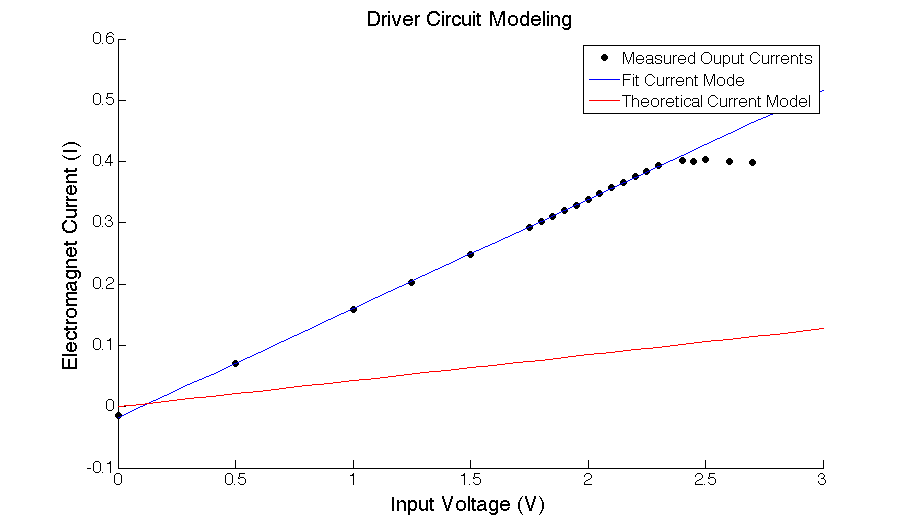
\includegraphics[width = 13cm]{DriverCircuitModel.png}
\label{Q1_d2}
\caption{\emph{Comparison of actual voltage current relationship with the fit model and the theoretical model}}
\end{center}
\end{figure}

\begin{table}
\begin{center}
    \begin{tabular}{|c|c|}
        \hline
        Component & Resistance ($\Omega$) \\ \hline
        $R_{1}$   & 46200                 \\ 
        $R_{2}$   & 999                   \\ 
        $R_{3}$   & 0.5                   \\
        \hline
    \end{tabular}
\caption{\emph{Measured Resistances in driver circuit.}}
\label{Q1_dt3}
\end{center}
\end{table}

\subsubsection*{Electromagnet}
$$ F(I,x) = \frac{A I^2}{(B+x)^2} $$
Examining our model for the force exerted by the electromagnet we see that we have two unknowns, A and B.  We conducted an experiment where we measured the amount of voltage sent to the driver to lift the steel sphere from a particular height.  We then attempted to perform non-linear optimization to determine A and B from this data however this computation diverged due to poor initial guesses for A and B.  To determine better initial guesses we symbolically solved for A and B as a function of two of these data points and then used these values as our initial estimate.  

At equilibrium we know that the force exerted by the electromagnet must balance out the force of gravity on the sphere, this yields the following two expressions.  In our experiment, the moment that the force exerted by the electro magnet exceeds the force of gravity, the sphere will stick to the magnet because the system was uncontrolled.  But in that moment we know that the system must have passed through the equilibrium current giving us a good measurement of the correct amount of current.
$$ mg = f = \frac{A I_{1}^2}{(B+x_{1})^2}  = \frac{A I_{2}^2}{(B+x_{2})^2} $$ 

We can solve the first expression for A.
$$ A = \frac{F (B + x_{1})^2}{I_{1}^2}$$

Then substituting the previous expression for A back into the $2^{nd}$ equation yields the following expression for B:
$$ B^2(1-R) + (2x_2-2x_1R)+x_2^2-x_1^2R = 0 \hspace{1cm} R = \frac{I_2^2}{I_1^1} $$

Choosing two of our x, I pairs allowed us to solve for plausible values of A and B which we used as initial guesses for the optimization allowing it to converge to the correct result.  Notice that because our model has both $I^2$ and $x^2$ terms, we expect multiple solutions for A and B.  The $I^2$ term physically means that the direction of current through the electromagnet is irrelevant to the force exerted.  However the x term is added to our B term before being squared.  Physically the B term prevents the force exerted by the electromagnet from going to infinity when x equals 0, but our model has no notion of notion of negative x values, even though it is perfectly legal to plug negative values in for x.  Small negative x values correspond to the steel sphere being within the magnet in real life, but in our model does not correctly handle this case.  In fact the model suggests that if B is a positive value then for some negative value for x the force exerted goes to infinity.  To handle these multiple solutions we attempted the optimization with both pairs of solutions and choose the one that minimized the overall error.  

 It is important to note the difference between the two different fits presented in figure \ref{Q1_d3}.  Both are the result of non-linear regression to solve for our unknown parameters A and B.  However the errors that each minimize is different.  The Current fit, minimizes the expected amount of current draw at each of our measured x values from the actual amount of current drawn by the electromagnet.  The Force fit minimizes the error between the expected amount of force, computed for each pair of observed current and position, and the actual amount of force required to lift the steel sphere.  The fit error described in table \ref{Q1_dt4} refers to the error in each fits respective space.  So the force fit has error in units of Newtons while the current fit has error in units of Amps so these two errors are not directly comparable.  The required current was computed assuming the specified amount of force needed.

Optimizing the error in force is the more correct answer for this problem because that is the error we wish to minimize. The force exerted is the dependent variable while the current and height are both independent variables.  Given a constant force we can link the height to the current, but this is only an approximation and assumes no external disturbances.  

\begin{figure}
\begin{center}
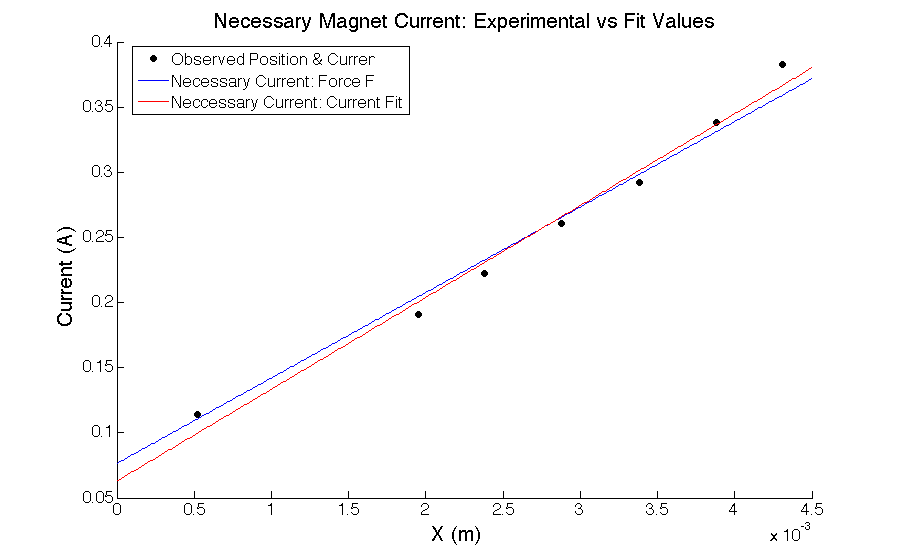
\includegraphics[width = 10cm]{magnetDataFits.png}
\label{Q1_d3}
\caption{\emph{Electromagnet Current vs X position}}
\end{center}
\end{figure}

\begin{table}
\begin{center}
    \begin{tabular}{|c|c|c|c|}
        \hline
        ~           & A          & B         &  Error \\ \hline
        Force Fit   & 2.2795e-05 & 0.0011656  & 0.0223076 N \\ 
        Current Fit & 1.9752e-05 & 8.9294e-04 & 0.0272997 A\\
        \hline
    \end{tabular}
\caption{\emph{Two different parameter fits to our data}}
\label{Q1_dt4}
\end{center}
\end{table}

\subsubsection*{Steel Sphere}
The steel sphere has two parameters of consequence for our modeling, its diameter and its mass.  Both of these values were obtained through direct measurements using calipers and a scale respectively shown in table \ref{Q1_dt5}.

\subsubsection*{Open Loop Transfer Function}
Substituting numerical values from our physical system yields the following open loop transfer function:
$$ \frac{-78511.7}{s^2 - 6201.6} $$

\begin{table}[hbt]
\begin{center}
    \begin{tabular}{|c|c|}
        \hline
        Steel Sphere Mass (g)      & 10   \\ \hline
        Steel Sphere Diameter (mm) & 12.7 \\
        \hline
    \end{tabular}
\caption{\emph{Steel sphere parameters}}
\label{Q1_dt5}
\end{center}
\end{table}


\subsection*{e.}
Figure \ref{Q1_e1}  shows the overall Simulink model of the nonlinear system, and figures \ref{Q1_e4} - \ref{Q1_e2} show the Simulink models of the individual sub-systems. The Matlab code for the non-linear model of the Photo-transistor can be seen in the appendix\footnote{Appendix: Matlab code for Photo-transistor: irradianceEstimator.m }.Figure \ref{Q1_e6}  shows the overall Simulink model of the linear system while figures \ref{Q1_e7} - \ref{Q1_e9} show the linearized Simulink models of the individual sub-systems.\\
\begin{figure}
\begin{center}
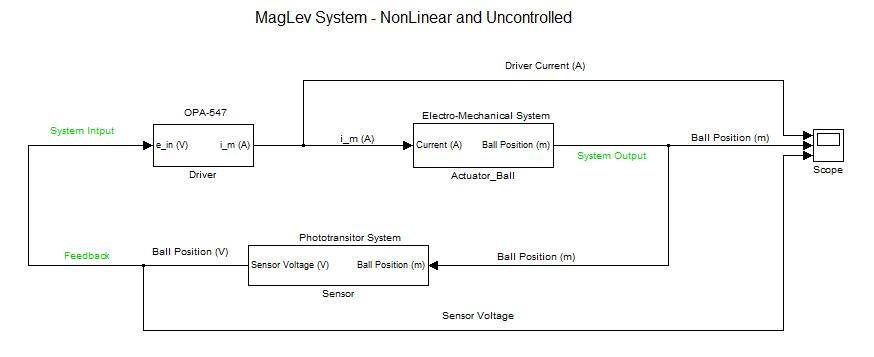
\includegraphics[width = 15cm]{NonLinearUnControlledComplete}
\caption{\emph{Nonlinear Simulink model}}
\label{Q1_e1}
\end{center}
\end{figure}

\begin{figure}
\begin{center}
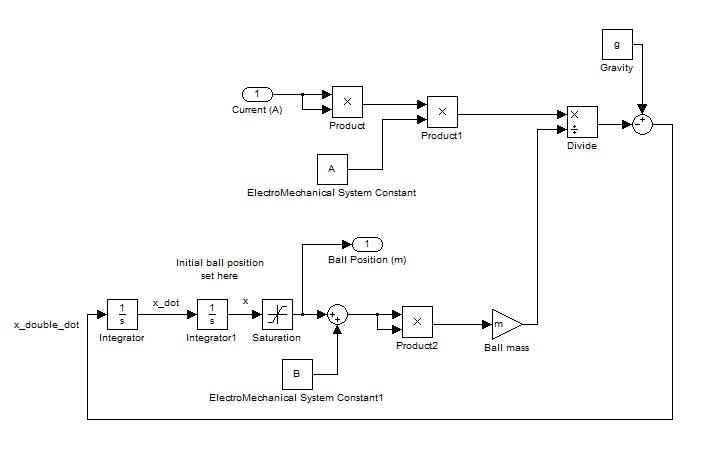
\includegraphics[width = 15cm]{NonLinearUnControlledActuatorBall}
\caption{\emph{Non-Linear Simulink model of Actuator-Ball Sub-System}}
\label{Q1_e4}
\end{center}
\end{figure}

\begin{figure}
\begin{center}
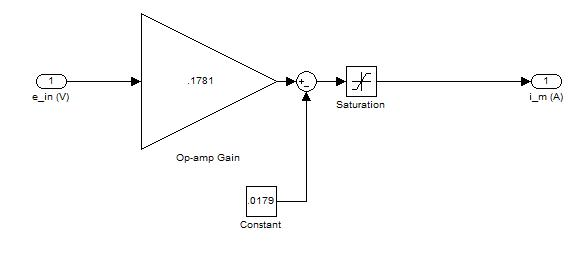
\includegraphics[width = 15cm]{NonLinearUnControlledDriver}
\caption{\emph{Non-linear Simulink model of the OPA-547 Op-Amp}}
\label{Q1_e5}
\end{center}
\end{figure}


\begin{figure}
\begin{center}
\includegraphics[width = 15cm]{NonLinearUnControlledPhototransistor}
\caption{\emph{Nonlinear Simulink model of the Phototransistor}}
\label{Q1_e2}
\end{center}
\end{figure}

%Linear.....

\begin{figure}
\begin{center}
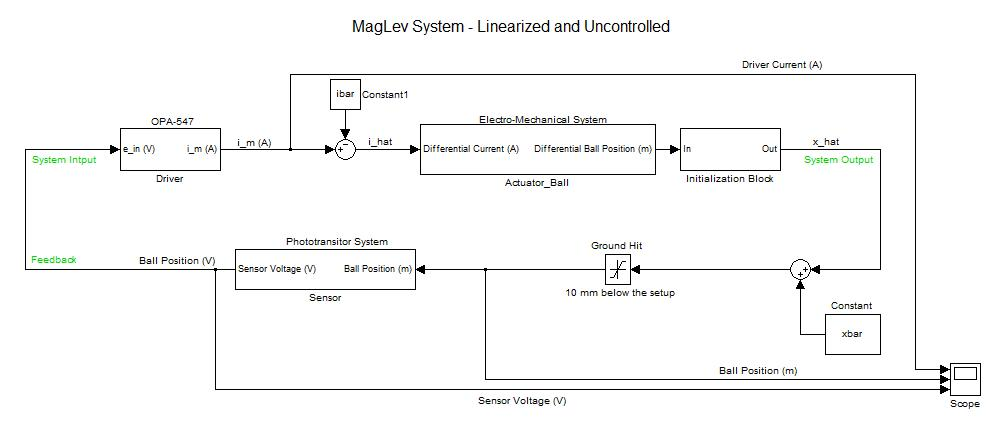
\includegraphics[width = 15cm]{LinearUnControlledComplete}
\caption{\emph{Linearized Simulink model}}
\label{Q1_e6}
\end{center}
\end{figure}

\begin{figure}
\begin{center}
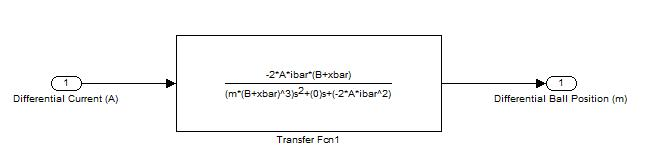
\includegraphics[width = 15cm]{LinearUnControlledActuatorBall}
\caption{\emph{Simulink model of the linearized Actuator-Ball Sub-System}}
\label{Q1_e7}
\end{center}
\end{figure}

\begin{figure}
\begin{center}
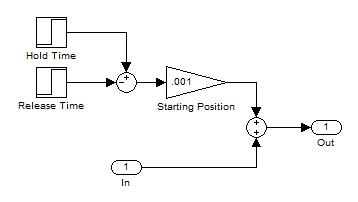
\includegraphics[width = 10cm]{LinearUnControlledInitialization}
\caption{\emph{Simulink Model of Initial Position Offset}}
\label{Q1_e8}
\end{center}
\end{figure}


\begin{figure}
\begin{center}
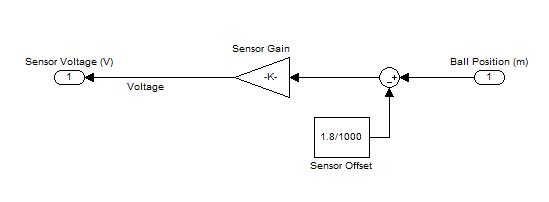
\includegraphics[width = 15cm]{LinearUnControlledSensor}
\caption{\emph{Linearized Simulink model of the Phototransistor}}
\label{Q1_e9}
\end{center}
\end{figure}



\subsection*{f.}
Figure \ref{Q1_f1} shows the time response of the nonlinear and linearized models when both are set to the nominal starting position ($\bar{x} = 0.00323$m). The time scale has been reduced to better show the behavior of both systems. In both cases the ball oscillates about a distance closer to the electromagnet than the starting point, with the ball in the nonlinear model ending up closer than the ball in the linearized model. In the case of the nonlinear model, the ball strikes the magnet before it begins oscillating, and the amplitude of its oscillations is less than the amplitude of the linearized model.\\
\begin{figure}[htb]
\begin{center}
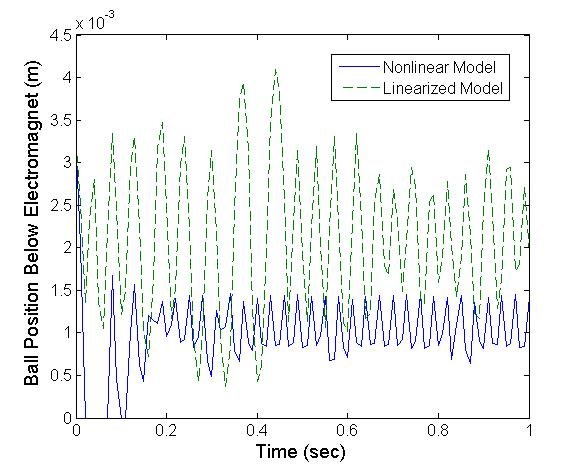
\includegraphics[width = 10cm]{Part1fNoDisturbance}
\caption{\emph{At the nominal starting height, both systems are able to levitate the ball, but also show sustained oscillations }}
\label{Q1_f1}
\end{center}
\end{figure}

In figure \ref{Q1_f2}, the nonlinear and linearized models are both set to a position one mm above the nominal starting position. The time scale has been reduced to better show the behavior of both systems. The linearized model again oscillates about a distance closer to the electromagnet than the starting point, but with smaller amplitude than previously. In the case of the nonlinear model, the ball strikes the magnet, is released, is re-attracted to the magnet, and then falls away.\\

\begin{figure}
\begin{center}
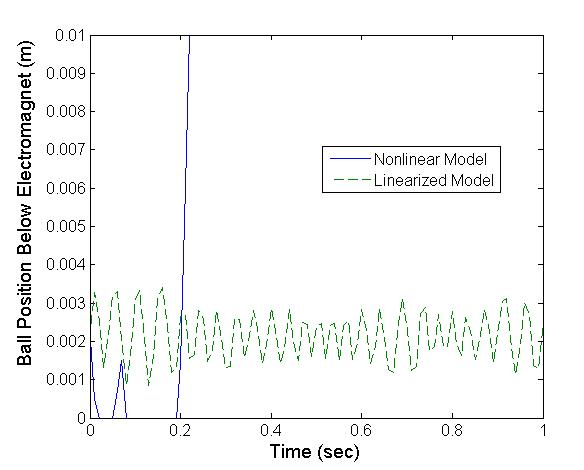
\includegraphics[width = 10cm]{Part1fCloseDisturbance}
\caption{\emph{When starting 1 mm further away from the electromagnet, the linearized model again predicts that it can still levitate the ball (with sustained oscillations) while the non-linear model again forecasts that the ball will fall}}
\label{Q1_f2}
\end{center}
\end{figure}

In figure \ref{Q1_f3}, the nonlinear and linearized models are both set to a position one mm below the nominal starting position. The time scale has been reduced to better show the behavior of both systems. The behavior here is very similar to the previous case. The linearized model oscillates about a distance closer to the electromagnet than the starting point, but with greater amplitude than with the closer starting point. The ball in the nonlinear model again strikes the magnet, and is then released and falls away.  

\begin{figure}[htb]
\begin{center}
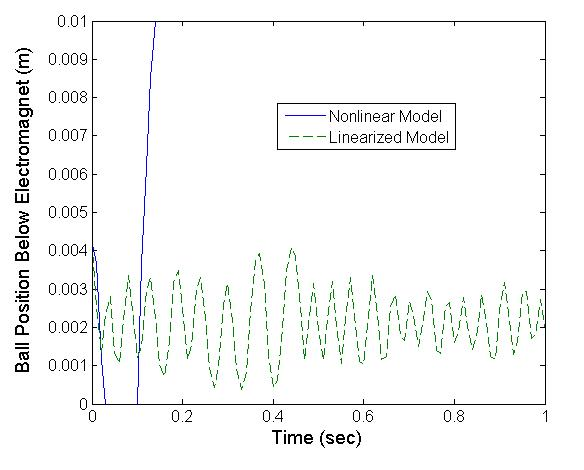
\includegraphics[width = 10cm]{Part1fFarDisturbance}
\caption{\emph{When starting 1 mm closer to the electromagnet, the linearized model predicts that it can still levitate the ball (with sustained oscillations) while the non-linear model forecasts that the ball will fall}}
\label{Q1_f3}
\end{center}
\end{figure}

When starting at the nominal position, the two models exhibit the same general behavior. However, changing the start point by greater than 0.01mm causes the nonlinear model to become unstable and fall away, while the linear model remains stable.As the model is uncontrolled, we expect the system to be unstable. However, the linearized model does not include the squared current and distance terms, so it is more \emph{optimistic} in terms of keeping the system stable. While the linearization does not agree with the nonlinear model over a large range, the general behavior is similar very close around our set point. Therefore, we believe our linearization assumptions are sufficient for the model, and the addition of a controller will improve the agreement between the models.

\subsection*{g.}

\section*{Question 2}
Using the linearized model from question one, the root locus plot in figure \ref{Q2} shows that the physical system will always be unstable in open-loop, because there will always be a pole in the right-half plane (RHP).\\

\begin{figure}[h!]
\begin{center}
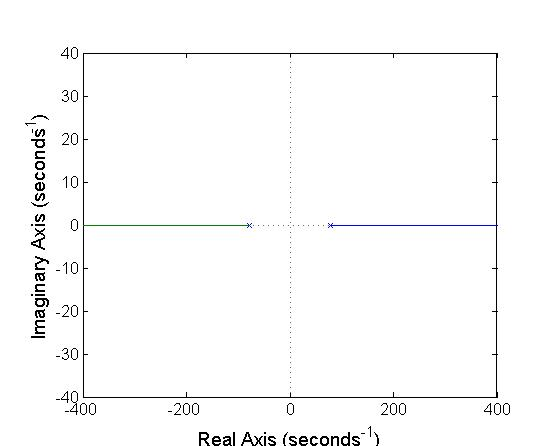
\includegraphics[width = 12cm]{FigureA}
\caption{\emph{Open-Loop Physical System is Always Unstable.}}
\label{Q2}
\end{center}
\end{figure}

A lead controller adds a pole and a zero to the system, with the pole being greater in magnitude than the zero (i.e. further from the imaginary axis) and both in the left-half plane (LHP). Because there were no design requirements given (settling time, overshoot, etc.), specific values were not as critical as they may have been otherwise, and we chose our controller pole to be at -80 and the controller zero to be at -20. Additionally, to ensure the proper sign throughout the system, a factor of -1 was applied to the controller. The root locus plot below shows the result of applying the controller to the system. We see that the system will be stable if the gain is large enough, because all of the closed-loop poles will be within the LHP. The gain magnitude must be greater than 0.096 for the rightmost pole to cross into the LHP, and greater gains reduce the settling time and steady-state error. But as the gain increases, the imaginary poles move further away from the real axis (lower damping). Therefore, we selected a gain of 0.37 as a compromise value. Our lead compensator is given by the equation below, and its effect on the physical system is shown in the following plot (figure \ref{Q2}). 

$$C(s)= -0.37 \frac{(s+20)}{(s+80)}$$

\begin{figure}[h!]
\begin{center}
\includegraphics[width = 12cm]{FigureB}
\caption{\emph{With Sufficient Gain, Lead Controller Stabilizes the System.}}
\label{Q2}
\end{center}
\end{figure}

\subsection*{a.}
From the root locus plot and Matlab sisotool analysis, the system must have a gain greater than 0.096 in magnitude (-20.35 dB). As mentioned previously, this gain must be negated to ensure the proper sign of the signal in the system. With the controller, $C(s)$, the closed-loop transfer function is given by:
$$\frac{2.367*10^4 s+ 4.732*10^5}{s^3+ 79.995 s^2+1.746*10^4 s - 2.290*10^4}$$

\begin{figure}[htb]
\begin{center}
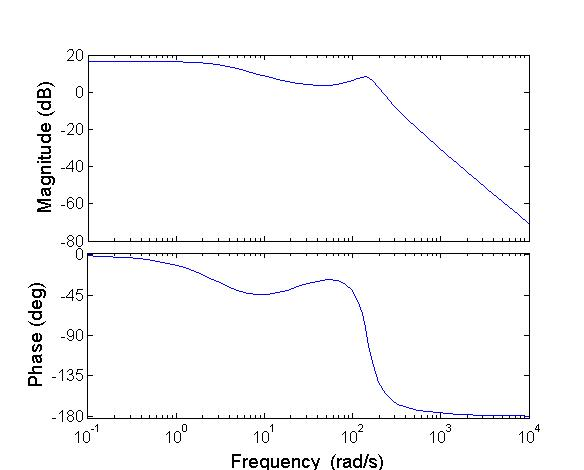
\includegraphics[width = 12cm]{ClosedLoopBode2}
\caption{\emph{Bode Plot of the Closed-Loop System.}}
\label{Q2_a}
\end{center}
\end{figure}

From the closed-loop bode plot(figure \ref{Q2_a}), the bandwidth (frequency at which the magnitude is -3 dB) is expected to be 468.22 rad/sec (74.52 Hz).

\subsection*{b.}
Figures \ref{Q2_b1} and \ref{Q2_b2} show the Simulink models of the nonlinear and linearized models, respectively, with the controller applied. Figure \ref{Q2_b3} shows the Simulink model of the controller itself, which is the same for the linearized and nonlinear models. All other sub-systems in the model are the same as shown in Part \emph{1 (e)}.\\

\begin{figure}[h!]
\begin{center}
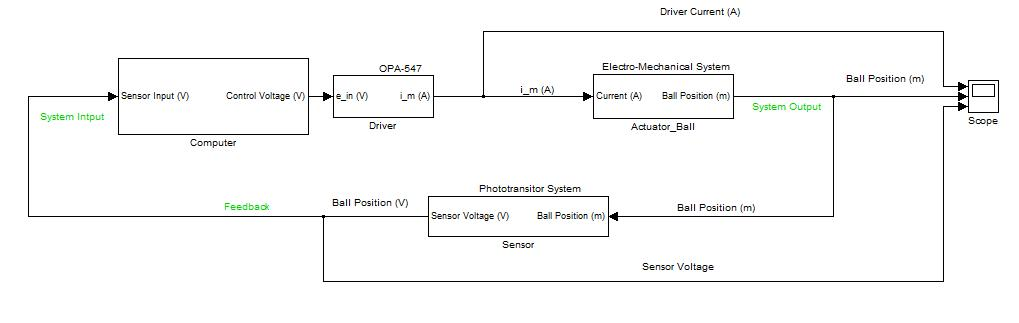
\includegraphics[width = 14cm]{NonLinearControlledComplete}
\caption{\emph{Nonlinear Model with Controller}}
\label{Q2_b1}
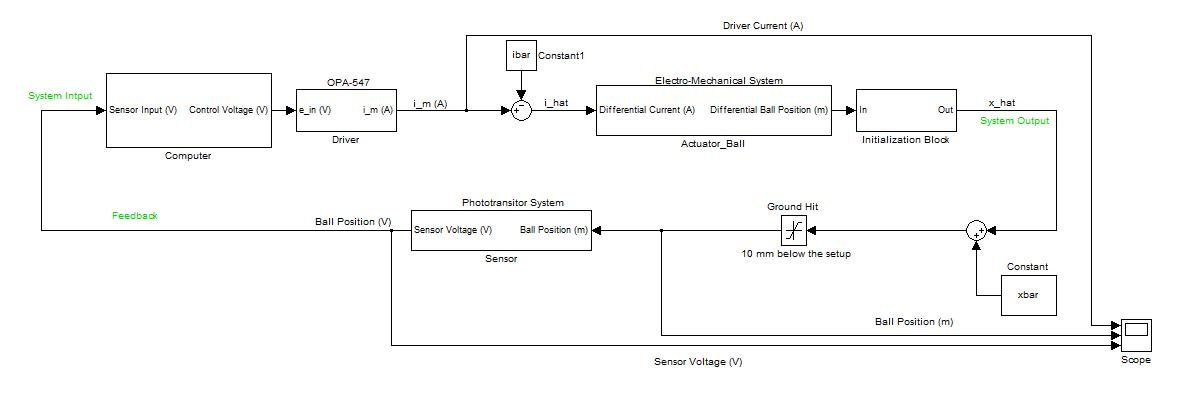
\includegraphics[width = 14cm]{LinearControlledComplete}
\caption{\emph{Linear Model with Controller}}
\label{Q2_b2}
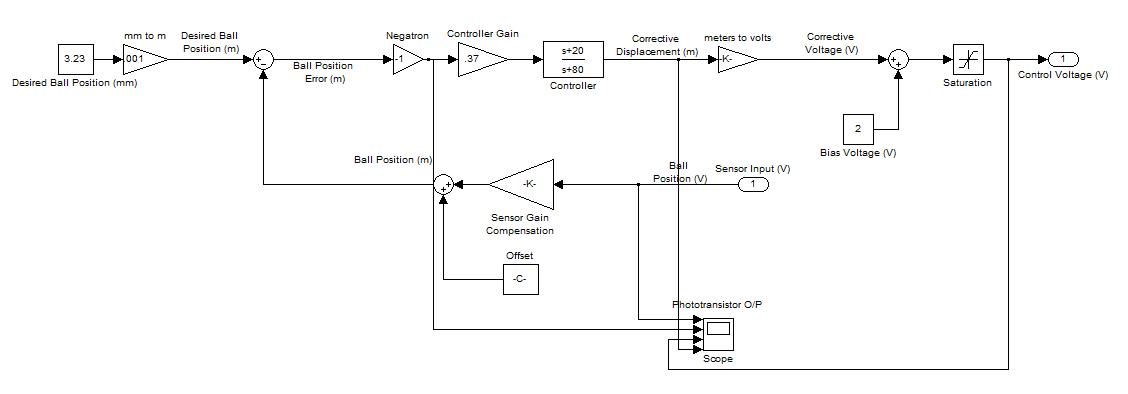
\includegraphics[width = 14cm]{Controller}
\caption{\emph{Simulink Model of the Controller sub-system}}
\label{Q2_b3}
\end{center}
\end{figure}

Figure \ref{Q2_b4} shows the time response of both models when the ball is started at the nominal height ($\bar{x} = .00323m$). Unlike the uncontrolled systems which oscillated continuously, when the controller is applied both systems settle on a steady position levitated below the electromagnet (the nonlinear model has some initial oscillations before settling).\\

\begin{figure}[h!]
\begin{center}
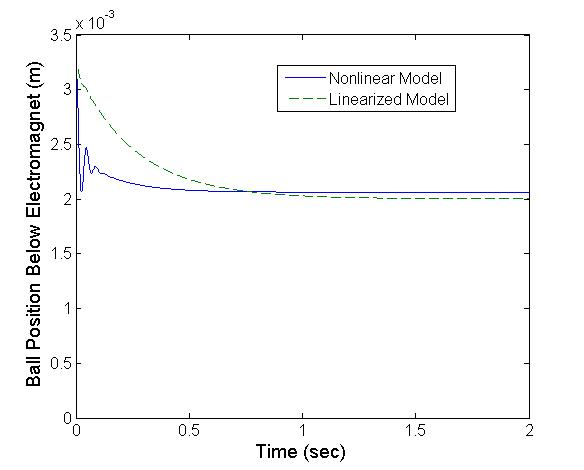
\includegraphics[width = 10cm]{Part2bNoDisturbance}
\caption{\emph{With the controller, both models have steady levitation positions when starting at the nominal distance.}}
\label{Q2_b4}
\end{center}
\end{figure}

If the starting position of the ball is moved closer to the magnet, both systems remain stable until a position 0.8mm above the set point, when the linearized model becomes unstable. An example of this is shown in figure \ref{Q2_b5}. In contrast, when the starting position is moved away from the magnet both systems remain stable until a position 1.9mm below the set point, when the nonlinear model becomes unstable. An example of this is shown in figure \ref{Q2_b6}.\\

\begin{figure}[h!]
\begin{center}
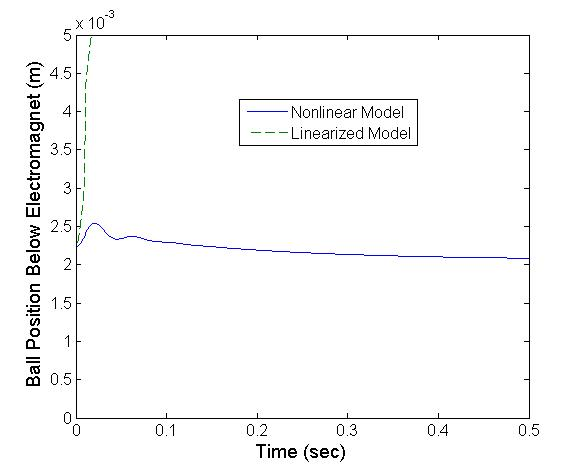
\includegraphics[width = 10cm]{Part2bCloseDisturbance}
\caption{\emph{When starting 0.8mm above the set point, the linearized model is unstable and the ball falls.}}
\label{Q2_b5}
\end{center}
\end{figure}

\begin{figure}[h!]
\begin{center}
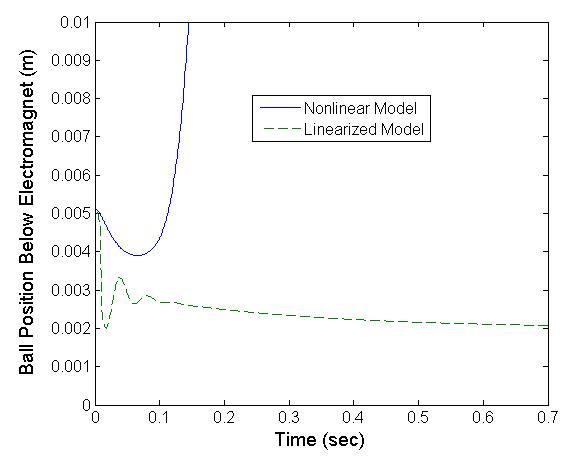
\includegraphics[width = 10cm]{Part2bFarDisturbance}
\caption{\emph{When starting 1.9mm below the set point, the nonlinear model is unstable and the ball falls.}}
\label{Q2_b6}
\end{center}
\end{figure}

Within the region where both models are stable, their overall behavior is similar, with both undergoing some oscillations before settling at different steady state points (the steady-state values are within 0.1mm of each other). The main difference between the models is that the linear model has a longer settling time, regardless of whether the starting point is above or below the set point. Another major difference is that when the start point is moved closer to the electromagnet, the linear model becomes unstable first, on the other hand, it is the nonlinear model that becomes unstable first when the start point is moved further from the electromagnet. 

\subsection*{c.}
The controller above does match the controller we used in the lab exercise during the previous week. Initially we had designed a new controller for this exercise, with different pole and zero locations, and a different gain value. However, both the nonlinear and linearized Simulink models were unstable under all of the conditions and variations we attempted. After discarding the new values and using the same poles, zeros, and gains that we had implemented in LabView on the test apparatus, the models became stable. This may be because prior to designing the controller for LabView, we conducted numerous tests to identify the parameters of the real system and modeled the various sub-systems. 

\subsection*{d.}
The block diagram in figure \ref{Q2_d} illustrates how we ensure we have negative feedback in our system. If we start at the far right and assume that the ball just moved slightly above the set point (closer to the electromagnet), the sensor outputs a voltage related to this position which will always be positive. This voltage is then converted to position (m) and subtracted from the set point. Because the ball is above the set point, the error will be positive. The error signal then passes through a gain block of -1 to flip its sign to negative. The controller takes in the negative error and outputs a negative voltage. By adding this negative voltage to the bias voltage, a lower command voltage is sent to the driver than previously (the starting assumption was that the ball had been at the setpoint, but just moved up). This results in a smaller current being sent to the actuator, which results in less force from the electromagnet. Less force from the electromagnet results in the ball falling further away from the magnet, back towards the set point. This is the behavior that we want.

\begin{figure}[h!]
\begin{center}
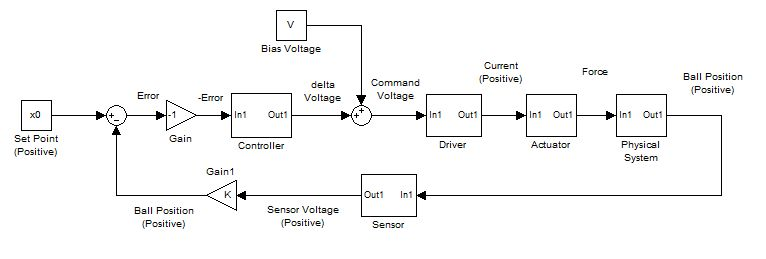
\includegraphics[width = 15cm]{BlockDiagram}
\caption{\emph{Block Diagram of System: Signs Ensure Negative Feedback.}}
\label{Q2_d}
\end{center}
\end{figure}


Similarly, if the ball is below the setpoint, the error will negative, and the inverting unity gain block will send a positive error into the controller, which will then output a positive voltage. Adding this voltage to the bias voltage results in a larger command voltage than when the ball is at the set point, so the current to the actuator will increase. The increased current will result in a larger force from the electromagnet, which will pull the ball back up towards the set point. Again, this is the behavior we want, so the signs within our system are correct. Because the physical and electronic sub-systems have restrictions on their signs (e.g. the sensor is tuned to always output between 0 and 10 volts), inserting the negation before the controller is the most important step to ensure we have stabilizing feedback. 

\section*{Question 3}

\newpage
\section*{Appendix}
\subsection*{Matlab code: radianceDerivative.m}
\begin{verbatim}
function [dRdd] = radianceDerivative(rbeam, rsphere, d)
% compute derivative of the radiance curve at a particular distance

assert((rbeam >= 0) && (rsphere >= 0), 'Expected non-negative numbers')

if ((rsphere + abs(d)) <= rbeam)
    % handle the block is completely in the beam and the beam is bigger
    dRdd = 0;
    
elseif ((rbeam + abs(d)) <= rsphere)
    % handle case where block is larger or same size than beam and completely in the way
    dRdd = 0;
    
elseif (abs(d) < (rbeam + rsphere))
    Abeam = pi * rbeam * rbeam;
    
    % y stuff
    y = (d*d + rbeam*rbeam - rsphere*rsphere) / (2 * d);
    dydd = 1/2 - (rbeam*rbeam)/(2*d*d) + (rsphere * rsphere) / (2*d*d)
    
    % intersection distances
    dbeam = y;
    ddbeam = dydd
    dsphere = d - y;
    ddsphere = 1 - dydd
    
    % occluded areas
    AObeam = cSarea(rbeam,dbeam)
    dAObeam = cSDarea(rbeam, dbeam, ddbeam)
    AOsphere = cSarea(rsphere,dsphere)
    dAOsphere = cSDarea(rsphere, dsphere, ddsphere)
    
    % total overlap
    AOverlap = AObeam + AOsphere;
    dAOverlap = dAObeam + dAOsphere;
    
    % change in radiance fraction
    dRdd = dAOverlap / Abeam;
else
    % handle if they aren't even touching
    dRdd = 0;
end

end

function [area] = cSarea(r, h) 
% computes the area of the circular segment where the upper boundary is a
% circular arc and the lower boundary is a cord of the circle with radius r
% h is the perpendicular distance from the center to the cord

area = r * r * acos(h / r) - h * sqrt(r * r - h * h);

end

function [dA] = cSDarea(r, h, dh)
dA = (- (r / sqrt(1 - (h/r)^2)) - sqrt(r*r - h*h) + ((h*h) / sqrt(r*r - h*h)))*dh;
end
\end{verbatim}

\subsection*{Matlab code for Photo-transistor: irradianceEstimator.m }
\begin{verbatim}
function irradianceRatio  = irradianceEstimator( x)
% computes the fraction of irradiance as a function of the radii of the two
% intersecting circles and the distance between their centers, d
% This can be used to model the irradiance of our phototransistor if we
% make several assumptions:
% - ignore diffraction
% - assume parallel light rays from LED to photo transistor so that we can
% model the * note we should use the minimum radius of the LED and the
% phototransistor - since - the parallel ray assumption means that distance
% from the ball to the LED doesn't matter

% let r1 be the beam radius and r2 be the blocking radius

% details at http://mathworld.wolfram.com/Circle-CircleIntersection.html

% estimated rblock = 6.35 mm
% estimated rbeam as = 2.3650 mm radius of the phototransistor

% regressed rbeam = 1.5048

%assert((rbeam >= 0) && (rblock >= 0), 'The radii should be non-negative');

r1 = (1.5048/1000);
r2 = (6.35/1000);

d = x + 4.12/1000;      % - (2.23/1000) + 12.7/2000;

if ((r1 > r2) && ((r2 + abs(d)) < r1))
    % handle the block is completely in the beam and the beam is bigger
    A1 = pi * r1 * r1;
    A2 = pi * r2 * r2;
    
    irradianceRatio = (A1 - A2) / A1;
    
elseif ((r2 >= r1) && ((r1 + abs(d)) <= r2))
    % handle case where block is larger or same size than beam and completely in the way
    irradianceRatio = 0;
        
elseif (abs(d) < (r1 + r2))
    % handle case where two circles intersect each other
    x = (d * d + r1 * r1 - r2 * r2) / (2 * d);
    
    d1 = x;
    d2 = (d * d - r1 * r1 + r2 * r2) / (2 * d);
    
    A = cSarea(r1, d1) + cSarea(r2, d2);
    
    Amax = pi * r1 * r1;
    
    irradianceRatio = (Amax - A) / Amax;

else 
    % handle case with no overlap
    irradianceRatio = 1;
end

end

function [area] = cSarea(r, h) 
% computes the area of the circular segment where the upper boundary is a
% circular arc and the lower boundary is a cord of the circle with radius r
% h is the perpendicular distance from the center to the cord

area = r * r * acos(h / r) - h * sqrt(r * r - h * h);

end
\end{verbatim}


\end{document}